\documentclass[a4paper,11pt]{article}
\usepackage[margin=1in]{geometry}
\usepackage{array}
\usepackage{booktabs}
\usepackage{caption}
\usepackage[english]{babel}
\usepackage[utf8]{inputenc}
\usepackage{amsmath}
\usepackage{graphicx}
\graphicspath{ {images/} }
\setlength{\headheight}{34.5pt}
\usepackage{fancyhdr}
\pagestyle{fancy}
\captionsetup{font=small,labelfont=bf}

\title{Revisiting the Gap--Shock--Reversal Pattern in Indian Corporate Bonds: Pandemic and Duration Checks}
\author{Rajal Lunkad\\23172}
\date{}

\begin{document}
\maketitle
\thispagestyle{empty}

\tableofcontents
\newpage

\section{General Problem Area}
Pricing and portfolio valuation usually treat the last observed price as current. For many corporate bonds this is not true: a bond can go days, weeks or months without trading, so its last price may be out of date when it trades again. The new yield then mixes several things: news that arrived while nobody was trading, a move in general interest rates, a change in the extra yield investors want for holding a bond that is hard to sell, and noise from a single trade. Corporate bond yields are known to contain a liquidity component \cite{chen2007corporate,bao2011illiquidity}, so a yield jump after a silence cannot be read as pure news.\\ \cite{kumar2026delayed} studies this in the Indian market using NSE trades from 2019 to 2026. The paper reports that longer silences are followed by larger yield jumps, and that large positive jumps partly reverse over the following weeks. This matters because it affects how far a last-traded price can be trusted as a mark for valuation.

\section{Research Question}
How much of this pattern is specific to bonds and to silence, and how much comes from something else? I examine two extensions of the design in \cite{kumar2026delayed}.
\begin{enumerate}
	\item \textbf{COVID-19:} Did the link between the trading gap and the size of the yield shock, and the link between the shock and the following 20-day excess return, differ across four periods (pre-COVID, crisis, recovery, post-recovery)?
	\item \textbf{Duration:} Does the link between the shock and the following 20-day excess return depend on the bond's modified duration?
\end{enumerate}
This report is an extension of \cite{kumar2026delayed} on a related but different dataset (Table~\ref{tab:replication}), not an independent discovery. Its contribution is modest: it shows how much of the pandemic and duration patterns can be traced to the government benchmark and to the way the return is defined.

\iffalse
\section{Literature Review}
Corporate bond yields contain a liquidity component on top of credit and interest-rate risk. Chen, Lesmond and Wei \cite{chen2007corporate} find that less liquid U.S. corporate bonds have higher yield spreads after controlling for bond, firm and macroeconomic variables. Bao, Pan and Wang \cite{bao2011illiquidity} find that corporate bonds are more illiquid than bid--ask spreads suggest and that market-wide illiquidity explains much of the time variation in the spreads of highly rated bonds. Dick-Nielsen, Feldh{\"u}tter and Lando \cite{dicknielsen2012corporate} find that the illiquidity component rose sharply around the subprime crisis. These papers are the reason I do not read a post-silence yield jump as pure news, and they show that liquidity conditions change over time. \\ Other work separates liquidity as a priced risk from liquidity as an event for a single bond. Lin, Wang and Wu \cite{lin2011liquidity} find that bonds more exposed to aggregate liquidity risk earn higher returns. Ivashchenko \cite{ivashchenko2025infrequently} finds that bonds with a history of trading dry-ups earn an extra 10 to 20 basis points per month. Kumar \cite{kumar2026delayed} asks a narrower question: whether the yield shock at the moment a silent bond trades again predicts its return over the next weeks, and whether the length of the silence adds anything once the shock is known. It reports that longer silences are followed by larger government-adjusted shocks, that larger positive shocks are followed by higher duration-adjusted excess returns, and that for a given shock bonds that were silent for long do not reverse more than active bonds. I use this design. \\ On predictability and India, Hong, Lin and Wu \cite{hong2012corporate} find serial dependence in corporate bond index returns, which is a market-level result. Mukherjee \cite{mukherjee2019demystifying} finds that irregular trading weakens standard liquidity measures in Indian corporate bonds, one reason an event-based design suits this market. Rathi and Pradhan \cite{rathi:gsec} study yield spreads in Government of India bonds, the market used here for the benchmark.

None of the papers I reviewed tests whether the shock--return relationship in \cite{kumar2026delayed} is stable through COVID-19 or depends on duration. I did not review studies of bond-market liquidity during COVID-19, so I cannot say whether others have examined this.
\fi

\section{Theory}
The starting point is the same as in \cite{kumar2026delayed}: for a bond that trades rarely, the last price becomes an out-of-date signal, and the next trade has to absorb news that arrived in the meantime, any change in liquidity conditions, and ordinary noise. Two relationships are used throughout.
\begin{itemize}
	\item \textbf{H1 (gap to shock):} the longer a bond has gone without trading, the larger the size of the yield shock when it trades again.
	\item \textbf{H2 (shock to return):} after a large yield shock, the bond tends to partly reverse over the next 20 days, which shows up as a positive excess return after a positive shock.
\end{itemize}

\paragraph{What a positive H2 slope can mean?} A positive H2 slope does not by itself show delayed price discovery. \cite{kumar2026delayed} lists several explanations that can all produce it: delayed price discovery, temporary price pressure, transaction-price noise, and issuer news that the government adjustment does not remove. For example, if the re-entry trade happens to be priced too cheaply by chance, the shock is positive and the next trade is likely to be closer to the fair yield, so the yield falls and the return is positive even though the first trade carried no information. The data used here cannot separate these explanations, so we call H2 a reversal.

\paragraph{The pandemic angle:} COVID-19 was a market-wide shock to liquidity and interest rates. For H1, a lot of news arrives in a short time in a crisis, so a bond silent for 20 days in March 2020 misses more news than one silent for 20 days in a calm year, and I expect a steeper H1 slope. Part of this news is about government rates, which the adjustment removes, so the raw and the adjusted slopes may behave differently; this is why we report both. For H2, a shock is corrected only if dealers and investors are willing to trade against it, and they are expected less willing in a crisis, so the correction could be slower, weaker or noisier.

\paragraph{The duration angle:} Duration measures how much a bond's price changes when its yield changes. The excess return is minus duration times the residual yield change, so duration is built into the outcome: even if the residual yield change after a shock were the same for every bond, the H2 slope in price terms would be larger for long-duration bonds. A positive shock-by-duration interaction is therefore expected from arithmetic alone. A more interesting possibility is that long-duration bonds also behave differently in yield terms, for example because their value depends on cash flows far in the future and is harder to judge. This is tested by running the H2 regression in yield space, without the duration multiplier.

\section{Hypotheses}
\begin{description}
	\item[Hypothesis A1:] The H1 slope differs across the four periods and is steepest in the crisis, \emph{ceteris paribus}. I test this for the raw yield change and for the government-adjusted shock.
	\item[Hypothesis A2:] The H2 slope does not differ significantly across the four periods.
	\item[Hypothesis B1:] The interaction between modified duration and the shock in the regression of the 20-day excess return on the shock is positive and significant, \emph{ceteris paribus}.
	\item[Hypothesis B2:] The reversal is larger for long-duration bonds in yield terms, so the slope of the residual yield change on the shock is more negative for long-duration bonds. B1 alone could be arithmetic; B2 would show more.
\end{description}

\section{Definitions}
\paragraph{Event, gap, stale and active:} An event is a trade of a bond (identified by its ISIN) paired with the previous trade of the same bond. The trading gap is the number of calendar days between the two trades. The regressions use $\log(1+\text{Gap})$ because gaps are very skewed. An event is \emph{stale} if its gap is at least 20 days, the cutoff used in \cite{kumar2026delayed}, and \emph{active} if its gap is at most 5 days.

\paragraph{Government yield:} RBI publishes weekly the minimum and maximum yield of secondary-market outright trades in central government securities, grouped by the fiscal year in which the security matures; the data are based on CCIL trades \cite{rbidbie}. We use the midpoint of the minimum and maximum for the fiscal year (April to March) in which the bond matures, and the ``and above'' column for later maturity years. Each trade date is matched to the first weekly observation on or after it, provided one exists within 10 days.

\paragraph{Government-adjusted shock:} Let $Y_{i,t}$ be the bond's volume-weighted average yield at the new trade date ($t$), $Y_{i,t_0}$ its yield at the previous trade date ($t_0$), and $G_{i,t}$ the matched government yield. Then
\[
\text{Shock}_{i,t} = (Y_{i,t}-Y_{i,t_0}) - (G_{i,t}-G_{i,t_0}).
\]
A positive shock means the bond became cheaper relative to government securities. Yields are in percentage points.

\paragraph{20-day excess return:}
\[
ER_{i,t+20} = -D_{i,t}\,\bigl(\Delta Y_{i,t+20}-\Delta G_{i,t+20}\bigr),
\]
where $D_{i,t}$ is modified duration, $\Delta Y_{i,t+20}$ is the change in the bond's yield from the new trade to its last trade within the next 20 calendar days, and $\Delta G_{i,t+20}$ is the change in the matched government yield between the same dates. The bracketed term is the \emph{residual yield change}; it is the outcome in the yield-space version of H2. The return exists only if the bond trades again within 20 days.

\paragraph{Periods:} Pre-COVID (January 2019 to February 2020), crisis (March to December 2020), recovery (2021 and 2022), post-recovery (2023 to August 2026).

\paragraph{Modified duration:} Duration is Macaulay duration divided by $1+y/m$, computed from the bond's yield $y$, coupon rate, coupon frequency $m$ and years to maturity. The NSE security master has no coupon column, so the coupon rate is read from the bond's issue name (for example ``8.50\%''). If no coupon is found the bond is treated as a par bond (coupon equal to yield), if no frequency is given annual coupons are assumed, and zero-coupon bonds get a coupon of zero. Bonds whose computed duration is not positive or exceeds years to maturity plus one are given no duration. Accrued interest and convexity are ignored. For the duration groups, the H2 sample is split into three groups of equal size (G1 low, G2 mid, G3 high).

\section{Control Variables}
The baseline H1 and H2 regressions have no controls, like the baseline regressions in \cite{kumar2026delayed}. Three checks are used instead. Duration also enters the interaction model on its own, so the interaction does not pick up its plain effect. Security-type fixed effects (a separate intercept for each NSE security-type code) are added in one version of the interaction model, because types may cluster at different durations. Standard errors are clustered by ISIN, because the same bond appears in many events. The trading gap, traded value and credit ratings are not controlled for (Section~\ref{sec:limits}).

\section{Case Selection}\label{sec:case}
The unit of analysis is the consecutive-trade event. We use every event in the sample period (1 January 2019 to 31 August 2026) from the NSE Corporate Bond Market (CBM) bhavcopy instead of drawing a sample. A trade is kept if its volume-weighted yield is between 0.5\% and 20\%, its volume-weighted price is between 40 and 180, traded value is positive, and its ISIN starts with ``INE'' (company-issued bonds), after removing commercial paper and certificates of deposit using the security master. If a bond has two records on the same day, the last one is kept. An event is kept if the absolute yield change from the previous trade is below 5 percentage points. These filters follow \cite{kumar2026delayed}.\\ The shock needs the bond's maturity date, which comes from the NSE security master, and a government yield for the bond's maturity year within 10 days of both trade dates. It is therefore available for only 75,920 of the 311,667 events (24\%). The H2 and duration tests use 7,535 stale events that have a shock, a duration and another trade within 20 days.


\section{Data and Criteria for Verification}\label{sec:criteria}
\paragraph{Estimation:} All regressions are ordinary least squares with standard errors clustered by ISIN.
\begin{align}
|M_{i,t}| &= a + b\,\log(1+\text{Gap}_{i,t}) + \varepsilon_{i,t}, \label{eq:h1}\\
ER_{i,t+20} &= a + b\,\text{Shock}_{i,t} + \varepsilon_{i,t}, \label{eq:h2}\\
ER_{i,t+20} &= a + b_1\,\text{Shock}_{i,t} + b_2\,(\text{Shock}_{i,t}\times\tilde D_{i,t}) + b_3\,\tilde D_{i,t} + \varepsilon_{i,t}. \label{eq:int}
\end{align}
In~\eqref{eq:h1}, $M$ is one of four outcomes: the raw yield change on all events (A), the raw yield change on events with a shock (B), the government-adjusted shock (C), or the change in the government yield (D). Equations~\eqref{eq:h2} and~\eqref{eq:int} use stale events with a shock and a 20-day return, and $\tilde D$ is duration minus the sample mean (about 4.4 years), so $b_1$ is the slope for a bond of average duration. The yield-space version of~\eqref{eq:h2} replaces $ER_{i,t+20}$ by the residual yield change.

\paragraph{Tests:} To test for breaks across periods, we re-estimate~\eqref{eq:h1} and~\eqref{eq:h2} on all events with period dummies and period-by-slope interactions (base: pre-COVID). The slope test is a Wald test that the three slope interactions are jointly zero (3 degrees of freedom). The shuffled-shock placebo randomly reassigns the shock values among the stale events, re-estimates~\eqref{eq:h2}, and repeats this 500 times; the empirical $p$-value is roughly the share of shuffled slopes as large in absolute value as the real one (the smallest value reachable with 500 shuffles is about 0.002).

\paragraph{What would support the hypotheses.}
\begin{itemize}
	\item \textbf{A1:} the slope test for H1 rejects, and the crisis slope is the highest.
	\item \textbf{A2:} the slope test for H2 does not reject. This is weak evidence, because failing to reject is not the same as showing equality, especially with small samples in two periods.
	\item \textbf{B1:} the interaction in~\eqref{eq:int} is positive and significant, also with security-type fixed effects, and the group slopes rise with duration.
	\item \textbf{B2:} the yield-space slope is more negative for long-duration bonds than for short-duration bonds.
\end{itemize}
The hypotheses are contradicted by a non-significant or wrongly ordered result in the corresponding test.

\section{Data Sources}\label{sec:sources}
All data are public. They were downloaded with a Python script, and the event file and variables were built with a second script.
\begin{enumerate}
	\item \textbf{NSE CBM daily bhavcopy} \cite{nsecbm}: 1,609 daily files from 1 January 2019 to 31 August 2026, about 358,700 bond-day records with the volume-weighted average price and yield, last-trade price and yield, and traded value.
	\item \textbf{NSE CBM security master} \cite{nsecbm}: a single snapshot with maturity date, coupon frequency, issue name (from which the coupon is read), security type and issuer.
	\item \textbf{RBI Database on Indian Economy} \cite{rbidbie}: the weekly series on secondary-market outright transactions in government securities, based on CCIL trade book data, with the minimum and maximum yield for each maturity-year bucket.
\end{enumerate}

\section{Results}
\subsection{Sample and replication}
The CBM files hold about 358,700 daily bond records. After the filters in Section~\ref{sec:case} and dropping each bond's first trade, 311,667 events remain. About 68\% are in the post-recovery period, and the crisis period is the smallest (20,689 events). Table~\ref{tab:replication} compares my pooled estimates with \cite{kumar2026delayed}. The raw-yield H1 slope is nearly identical (0.0799 against 0.079). The adjusted-shock slope is a little smaller (0.064 against 0.071) on about 38\% fewer events. The H2 slope is larger than the paper's (0.95 against 0.57), but its sign and the asymmetry agree: reversal after positive shocks is much stronger than after negative ones. 

\begin{table}[htbp]
\centering
\caption{Comparison with Kumar \cite{kumar2026delayed}, pooled estimates.}
\label{tab:replication}
\footnotesize
\begin{tabular}{p{5.2cm}rrrrrr}
\toprule
 & \multicolumn{3}{c}{Kumar \cite{kumar2026delayed}} & \multicolumn{3}{c}{This report} \\
\cmidrule(lr){2-4}\cmidrule(lr){5-7}
Regression & $\beta$ & sample size & $R^2$ & $\beta$ & sample size & $R^2$ \\
\midrule
H1: raw $|\Delta Y|$, all events        & 0.079 & 308,215 & 0.050 & 0.0799 & 311,667 & 0.0511 \\
H1: adjusted $|\text{Shock}|$           & 0.071 & 122,933 & 0.045 & 0.0640 & 75,920  & 0.0347 \\
H2: $ER_{20}$ on shock, stale events    & 0.574 & 13,294  & 0.077 & 0.9474 & 7,535   & 0.0880 \\
H2: positive shocks only                & 0.824 & 6,920   & 0.099 & 1.4313 & 4,157   & 0.1265 \\
H2: negative shocks only                & 0.166 & 6,368   & 0.005 & 0.3742 & 3,378   & 0.0122 \\
\bottomrule
\end{tabular}
\end{table}

\subsection{H1 across periods (Hypothesis A1)}
Table~\ref{tab:h1} reports equation~\eqref{eq:h1} by period for the four outcomes. Columns B, C and D use the same 75,920 events, so they can be compared directly.

\begin{table}[htbp]
\centering
\caption{H1: slope $b$ of $|M|$ on $\log(1+\text{gap})$ by period (standard error in brackets, clustered by ISIN).}
\label{tab:h1}
\footnotesize
\setlength{\tabcolsep}{4pt}
\begin{tabular}{lrcrccc}
\toprule
 & \multicolumn{2}{c}{All events} & \multicolumn{4}{c}{Events with a shock} \\
\cmidrule(lr){2-3}\cmidrule(lr){4-7}
Period & sample size & A: raw $|\Delta Y|$ & sample size & B: raw $|\Delta Y|$ & C: adj.\ $|\text{Shock}|$ & D: $|\Delta G|$ \\
\midrule
Pre-COVID      & 28,118  & 0.1152 (0.0031) & 5,677  & 0.0642 (0.0043) & 0.0510 (0.0043) & 0.0759 (0.0022) \\
Crisis         & 20,689  & 0.1968 (0.0052) & 4,074  & 0.1094 (0.0053) & 0.0673 (0.0048) & 0.1037 (0.0042) \\
Recovery       & 50,992  & 0.1226 (0.0029) & 9,692  & 0.0754 (0.0038) & 0.0731 (0.0038) & 0.1015 (0.0021) \\
Post-recovery  & 211,868 & 0.0486 (0.0019) & 56,477 & 0.0345 (0.0037) & 0.0625 (0.0039) & 0.0918 (0.0017) \\
\midrule
All            & 311,667 & 0.0799 (0.0017) & 75,920 & 0.0467 (0.0031) & 0.0640 (0.0032) & 0.0933 (0.0013) \\
\bottomrule
\end{tabular}

\vspace{4pt}
\begin{minipage}{0.97\textwidth}\footnotesize\raggedright
\textit{Notes:} All $p$-values are below 0.0001. $\Delta Y$ is the bond's yield change since its previous trade, $\Delta G$ the change in the matched government yield, and Shock $= \Delta Y - \Delta G$.
\end{minipage}
\end{table}

Hypothesis A1 predicted that the slope is steepest in the crisis. It is for the raw yield change (A and B) and for the government yield move (D), for example 0.197 against 0.115 pre-COVID in column A. It is not for the adjusted shock (C): 0.0673 in the crisis against 0.0731 in recovery, a difference of about one standard error. The adjusted crisis slope is above the pre-COVID slope (0.0510), although the 95\% intervals ([0.058, 0.077] and [0.043, 0.059]) only just overlap. The adjustment lowers the slope more in the crisis than in the other periods: on the same events the adjusted slope is 79\% of the raw slope pre-COVID, 62\% in the crisis, 97\% in recovery and 181\% in post-recovery. These ratios compare slopes estimated on absolute values, so they are descriptive and not an exact decomposition. The post-recovery ratio above 100\% means the adjustment raises the slope there, which I cannot explain.

The slopes differ across periods. The Wald slope test (3 degrees of freedom) rejects for the raw yield change ($\chi^2 = 937.96$, $p < 0.0001$) and for the adjusted shock ($\chi^2 = 18.76$, $p = 0.0003$). The raw test uses four times as many events, which is part of why its statistic is so much larger; the break in the adjusted shock is smaller but still significant. On whether the link recovered: the raw post-recovery slope (0.0486) is less than half the pre-COVID slope (0.1152), but the adjusted slope shows no decline (0.0625 against 0.0510).

\textbf{Verdict on A1: partly supported.} The gap--yield link differs across periods. The 2020 spike is clear in raw yields and government yields, but the bond-specific part (the adjusted slope) rises less and is highest in recovery, not in the crisis. The pandemic effect on this relationship therefore operates largely through government yields.

\subsection{H2 across periods (Hypothesis A2)}
Table~\ref{tab:h2} reports equation~\eqref{eq:h2} by period. The pooled slope is 0.9474 ($t = 11.90$): a shock of one percentage point is followed by about 0.95 percentage points of excess return over the next 20 days. In yield terms (Table~\ref{tab:duration}) a one-point shock is followed by a fall of 0.28 points in the residual yield, so about 28\% of the shock reverses within 20 days. This is a partial reversal. The $R^2$ is 0.088, similar to the 0.077 in \cite{kumar2026delayed}.

The recovery slope (1.1137, $t = 6.71$) and the post-recovery slope (0.9707, $t = 10.70$) are strongly significant and close to each other. The pre-COVID slope (0.7485, $t = 1.72$) is significant only at the 10\% level and the crisis slope (0.3913, $t = 1.05$, $p = 0.29$) is not significant. These two rest on 379 and 409 events, and their 95\% intervals ([$-0.11$, 1.60] and [$-0.34$, 1.12]) include zero and also include the recovery and post-recovery slopes. The slope test does not reject equality ($\chi^2 = 3.14$, $p = 0.37$). A joint test that also lets the intercept differ does reject ($p < 0.0001$), so the average 20-day excess return differs across periods; I did not look into this.

The shuffled-shock placebo supports the pooled, pre-COVID, recovery and post-recovery slopes (empirical $p \le 0.018$), but not the crisis slope ($p = 0.114$): the real value (0.3913) is below the 95th percentile of the absolute shuffled slopes (0.4826), so shuffled data can easily give a slope this size. Dropping the five ISINs with the most events leaves the pooled slope almost unchanged (0.9504, $n = 7{,}365$), so a few frequently traded bonds do not drive the result.

\begin{table}[htbp]
\centering
\caption{H2: slope of $ER_{20}$ on the shock by period, for stale events (gap $\ge$ 20 days) and for active events (gap $\le$ 5 days) (standard error in brackets, clustered by ISIN).}
\label{tab:h2}
\footnotesize
\begin{tabular}{lrcrrc}
\toprule
 & \multicolumn{3}{c}{Stale events} & \multicolumn{2}{c}{Active events} \\
\cmidrule(lr){2-4}\cmidrule(lr){5-6}
Period & $n$ & $\beta$ (SE) & Shuffled-shock $p$ & $n$ & $\beta$ (SE) \\
\midrule
Pre-COVID      & 379   & 0.7485 (0.4362) & 0.0180 & 3,556  & 2.3643 (0.2444) \\
Crisis         & 409   & 0.3913 (0.3719) & 0.1138 & 2,117  & 3.6423 (0.4654) \\
Recovery       & 1,396 & 1.1137 (0.1660) & 0.0020 & 3,940  & 2.0150 (0.2700) \\
Post-recovery  & 5,351 & 0.9707 (0.0907) & 0.0020 & 31,271 & 1.0257 (0.0708) \\
\midrule
All            & 7,535 & 0.9474 (0.0796) & 0.0020 & 40,884 & 1.1396 (0.0763) \\
\bottomrule
\end{tabular}
\end{table}

\begin{figure}[htbp]
\centering
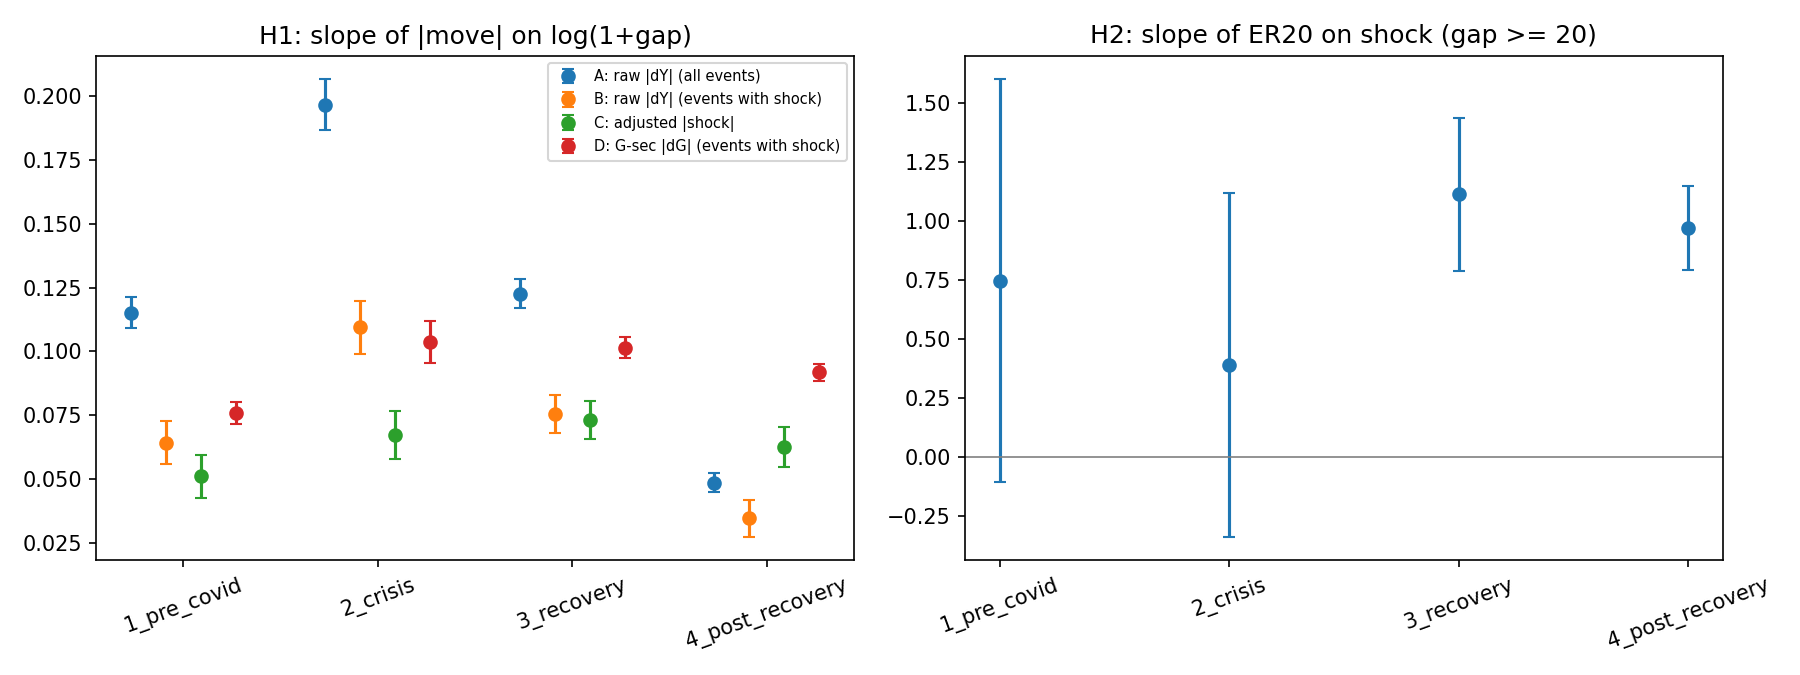
\includegraphics[width=\textwidth]{fig_h1_h2_by_window.png}
\caption{Left: H1 slopes by period for the four outcomes in Table~\ref{tab:h1}. Right: H2 slopes by period for stale events (Table~\ref{tab:h2}). Bars show 95\% confidence intervals clustered by ISIN.}
\label{fig:byperiod}
\end{figure}

\paragraph{Active bonds.} If H2 only happened after long silences, the slope should be weak for active bonds, which have little stale information to release. It is instead positive and significant in every period and larger than the stale-bond slope in the pooled sample (1.14 against 0.95); it is largest in the crisis (3.64). This is the same direction as Table 9 of \cite{kumar2026delayed}, where the shock coefficient is larger for active bonds (1.028) than for stale bonds (about 0.57). I did not test these differences formally. The implication is that H2 is not specific to bonds that were silent for a long time, so the H2 slope alone does not show that stale information is the cause.

\textbf{Verdict on A2: no evidence of a change, but low power.} The reversal is present and similar in 2021--2026, where it is precisely estimated. For the pre-COVID and crisis periods the estimates are too imprecise to say anything, and the crisis slope cannot be separated from noise by the placebo.

\subsection{Duration (Hypotheses B1 and B2)}
With mean-centred duration, the interaction in equation~\eqref{eq:int} is 0.1733 (SE 0.0381, $t = 4.55$, 95\% interval 0.099 to 0.248): each extra year of duration adds about 0.17 to the H2 slope. Adding security-type fixed effects changes it only to 0.1740 ($t = 4.57$), so the duration effect is not a security-type effect. The slope at average duration is 1.08 (SE 0.095) and the $R^2$ is about 0.10. With uncentred duration the interaction is identical, and only the shock coefficient changes, because it then refers to a bond with duration zero.

Table~\ref{tab:duration} gives the H2 slope within the three duration groups, in price space and in yield space.

\begin{table}[htbp]
\centering
\caption{H2 by duration group, stale events: price space ($ER_{20}$) and yield space (residual yield change) (standard error in brackets, clustered by ISIN).}
\label{tab:duration}
\footnotesize
\setlength{\tabcolsep}{4pt}
\begin{tabular}{lrrcc c}
\toprule
Group & Mean duration & $n$ & Price space: $ER_{20}$ slope & Yield space: slope & $-$(yield slope) $\times$ mean duration \\
\midrule
G1 low  & 2.12 & 2,512 & 0.6384 (0.0916) & $-0.3120$ (0.0370) & 0.66 \\
G2 mid  & 4.45 & 2,511 & 1.0977 (0.1281) & $-0.2616$ (0.0304) & 1.16 \\
G3 high & 6.75 & 2,512 & 1.4784 (0.2328) & $-0.2217$ (0.0375) & 1.50 \\
\midrule
All     & 4.44 & 7,535 & 0.9474 (0.0796) & $-0.2767$ (0.0222) & --- \\
\bottomrule
\end{tabular}

\vspace{4pt}
\begin{minipage}{0.97\textwidth}\footnotesize\raggedright
\textit{Notes:} All $p$-values are below 0.0001. Groups have equal size: G1 is 0.1141 to 3.3451 years, G2 3.3454 to 5.5673 years, G3 5.5685 to 12.1197 years. Mean durations are my approximations, computed from the means of the positive- and negative-shock subgroups in the output. The last column is the yield-space slope times the mean duration, to compare with the price-space slope.
\end{minipage}
\end{table}

\begin{itemize}
	\item \textbf{Price space.} The slope rises from 0.64 to 1.10 to 1.48, so G3 is about 2.3 times G1, and the 95\% intervals of G1 ([0.459, 0.818]) and G3 ([1.022, 1.935]) do not overlap. This agrees with the interaction (B1).
	\item \textbf{Yield space.} The coefficients are negative in every group, so shocks reverse, but they are not larger for long-duration bonds: $-0.31$, $-0.26$, $-0.22$, if anything slightly smaller. The 95\% intervals of G1 ([$-0.384$, $-0.240$]) and G3 ([$-0.295$, $-0.148$]) overlap, so I cannot say that the yield-space reversal differs by group (B2). I did not test the difference formally.
	\item \textbf{Arithmetic.} The yield-space slope times the group's mean duration gives 0.66, 1.16 and 1.50, within about 6\% of the price-space slopes (0.64, 1.10, 1.48). The rising slope in price terms therefore comes almost entirely from the duration multiplier.
	\item \textbf{Issuer concentration.} The five issuers with the most events (Indian Railway Finance Corporation, REC Ltd, Power Finance Corporation Limited, LIC Housing Finance Ltd. and Tata Capital Limited) account for 3,213 of the 7,535 events (43\%). Without them the price-space slopes are 0.66, 1.00 and 1.30, still rising, but the G3-to-G1 ratio falls from 2.3 to about 2.0.
\end{itemize}

\textbf{Verdict on B: B1 is supported, B2 is not.} The duration gradient in the excess-return slope is large and robust, but it is what the definition of the return implies. The data give no evidence that long-duration bonds correct shocks more strongly in yield terms.

\section{Discussion}
\paragraph{Pandemic.} The clearest pandemic result is that the 2020 jump in the gap--yield link is visible in raw yields and in the government yield move itself, but much less so in the government-adjusted shock. This points to a pandemic effect operating largely through government rates, and not to a sharp, temporary fall in bond-specific price discovery. The adjusted slope also does not return to its pre-COVID level by 2026, but the evidence for this is only as good as the government benchmark, which is coarse here (Section~\ref{sec:limits}).

\paragraph{The reversal.} About 28\% of a shock reverses in yield terms within 20 days, and the relationship is stable in the periods where it can be measured. What it means is less clear than a first reading suggests. The same reversal appears for actively traded bonds, so it is not specific to silence, and a pricing error at a single re-entry trade would produce the same pattern. Kumar \cite{kumar2026delayed} reports that the slope falls but stays positive when small trades are excluded (0.366 for traded value of at least Rs.~5 crore, against 0.574 overall); I did not run this check. I therefore treat H2 as a descriptive regularity and not as proof of delayed price discovery.

\paragraph{Duration.} For anyone comparing reversal across bonds, the practical point is that excess-return slopes are not comparable across durations, because duration is built into them. In yield terms the reversal is similar across duration groups. Studies of how reversal depends on bond characteristics should therefore be run in yield space, or should adjust for the multiplier.

\section{Limitations}\label{sec:limits}
\paragraph{Survivorship and calendar time.} The security master is a single September 2026 snapshot that lists only bonds still outstanding then, so bonds that matured earlier are missing and early events can only come from long-maturity bonds (Section~\ref{sec:case}). Differences between periods may therefore partly reflect different kinds of bonds, and the duration groups may differ in calendar time as well as in duration. I did not tabulate duration by period. Older snapshots would reduce the problem but would change all numbers.

\paragraph{Government benchmark.} The benchmark is weekly and reports only the minimum and maximum yield, so I use the midpoint. It is matched by maturity fiscal year and not by exact residual maturity, and each trade date is matched to the first weekly observation on or after it (within 10 days), so the benchmark can come from a few days after the trade. This is coarser than the NSE wholesale tape in \cite{kumar2026delayed} and may add noise to the shock. I cannot explain why the adjustment raises the slope in the post-recovery period.

\paragraph{Selection and noise.} The 20-day return exists only if the bond trades again within 20 days; in \cite{kumar2026delayed} only about half of stale events have such a trade, and bonds that do not trade again may differ. I cannot separate delayed price discovery from price noise or temporary price pressure, and the data have no bid--ask quotes. I did not run traded-value cuts.

\paragraph{Duration measurement.} The coupon is read from the issue name, with fallbacks (coupon equal to yield, annual frequency) when information is missing, and I did not count how many bonds used a fallback. Floating-rate and step-up bonds are not treated separately, and convexity and accrued interest are ignored. Duration also correlates with security type (47\% of DB events are in G1, while 42\% of PT and PF events are in G3), although security-type fixed effects leave the interaction unchanged (0.1733 to 0.1740).

\paragraph{Inference and design.} Standard errors are clustered by ISIN and not by date, so events on the same date, especially in March 2020, are treated as independent, which may make standard errors too small. The pre-COVID and crisis H2 samples are small (379 and 409 events), the H2 regressions do not control for the trading gap or traded value, no credit ratings were available, and many specifications were examined without correction for multiple testing. The shock exists for only 24\% of events. The design is observational: matching on government yields removes a benchmark component, but the residual shock may still contain credit news. All results are associations, not causal effects.

\section{Conclusion}
I extended the event design of \cite{kumar2026delayed} to ask whether the gap--yield link (H1) and the shock--return link (H2) changed with COVID-19 and whether the reversal depends on duration. Three findings are best supported. First, the gap--yield link differs significantly across periods, but the 2020 spike is largely a raw-yield and government-yield effect, and the adjusted slope is not highest in the crisis. Second, about 28\% of a shock reverses in yield terms within 20 days, but this also happens for actively traded bonds, so it does not isolate silence, and the crisis estimate is too imprecise to interpret. Third, the excess-return reversal rises with duration, but the yield-space reversal does not, so this gradient is almost entirely the duration multiplier.

These results are limited by survivorship in the security master, selection into re-trading, a coarse weekly benchmark, and the possibility that the reversal reflects price noise. The next steps that would most improve the work are: older security master snapshots with a table of duration by period; traded-value checks for H2; clustering by date; a formal test of whether the yield-space slopes differ across duration groups; and a daily government benchmark.

\clearpage
\begin{thebibliography}{99}
\bibitem{kumar2026delayed}
Kumar, G. ``Delayed Price Discovery and Return Adjustment in Indian Corporate Bonds.'' Working paper (SSRN draft), 2026. Draft covering NSE Corporate Bond Market data, 1 January 2019 to 27 August 2026.

\bibitem{chen2007corporate}
Chen, L., Lesmond, D. A., and Wei, J. (2007). Corporate yield spreads and bond liquidity. \emph{Journal of Finance}, 62(1), 119--149.

\bibitem{bao2011illiquidity}
Bao, J., Pan, J., and Wang, J. (2011). The illiquidity of corporate bonds. \emph{Journal of Finance}, 66(3), 911--946.

\bibitem{dicknielsen2012corporate}
Dick-Nielsen, J., Feldh{\"u}tter, P., and Lando, D. (2012). Corporate bond liquidity before and after the onset of the subprime crisis. \emph{Journal of Financial Economics}, 103(3), 471--492.

\bibitem{lin2011liquidity}
Lin, H., Wang, J., and Wu, C. (2011). Liquidity risk and expected corporate bond returns. \emph{Journal of Financial Economics}, 99(3), 628--650.

\bibitem{hong2012corporate}
Hong, Y., Lin, H., and Wu, C. (2012). Are corporate bond market returns predictable? \emph{Journal of Banking and Finance}, 36(8), 2216--2232.

\bibitem{ivashchenko2025infrequently}
Ivashchenko, A. (2025). (In)Frequently traded corporate bonds and pricing implications of liquidity dry-ups. \emph{Finance Research Letters}, 75, 106880.

\bibitem{mukherjee2019demystifying}
Mukherjee, K. N. (2019). Demystifying yield spread on corporate bonds trades in India. \emph{Asia-Pacific Financial Markets}, 26(2), 253--284.

\bibitem{rathi:gsec}
Rathi, K., and Pradhan, H. K. Determinants of yield spread in the Government of India bond markets. Working paper, SSRN.

\bibitem{rbidbie}
Reserve Bank of India. Secondary Market Outright Transactions in Government Securities (Face Value), Database on Indian Economy (DBIE). Weekly data based on the trade book of the Clearing Corporation of India Ltd. (CCIL). Accessed September 2026.

\bibitem{nsecbm}
National Stock Exchange of India. Corporate Bond Market (CBM) Bhavcopy and Security Master. Accessed via nseindia.com/api/reports, September 2026.
\end{thebibliography}

\end{document}
